%
% The MIT License (MIT)
%
% Copyright (c) 2017 Paul Batty
%
% Permission is hereby granted, free of charge, to any person obtaining a copy
% of this software and associated documentation files (the "Software"), to deal
% in the Software without restriction, including without limitation the rights
% to use, copy, modify, merge, publish, distribute, sublicense, and/or sell
% copies of the Software, and to permit persons to whom the Software is
% furnished to do so, subject to the following conditions:
%
% The above copyright notice and this permission notice shall be included in
% all copies or substantial portions of the Software.
%
% THE SOFTWARE IS PROVIDED "AS IS", WITHOUT WARRANTY OF ANY KIND, EXPRESS OR
% IMPLIED, INCLUDING BUT NOT LIMITED TO THE WARRANTIES OF MERCHANTABILITY,
% FITNESS FOR A PARTICULAR PURPOSE AND NONINFRINGEMENT. IN NO EVENT SHALL THE
% AUTHORS OR COPYRIGHT HOLDERS BE LIABLE FOR ANY CLAIM, DAMAGES OR OTHER
% LIABILITY, WHETHER IN AN ACTION OF CONTRACT, TORT OR OTHERWISE, ARISING FROM,
% OUT OF OR IN CONNECTION WITH THE SOFTWARE OR THE USE OR OTHER DEALINGS IN
% THE SOFTWARE.
%

\section{Architecture}

Now that the paper has covered all the concepts and ideas needed to build a full continuous deployment pipeline, this next section aims to look at the different form found in use and how they are put together.

\subsection{Starting point}

So far the paper has mentioned about a pipeline, the pipeline being taking the developers changes and getting then out to the customer in a working order. From a purely simplistic point of view the pipeline will look like the that seen in figure \ref{fig:pipeline-simple}.

\begin{figure}[H]
	\centering
	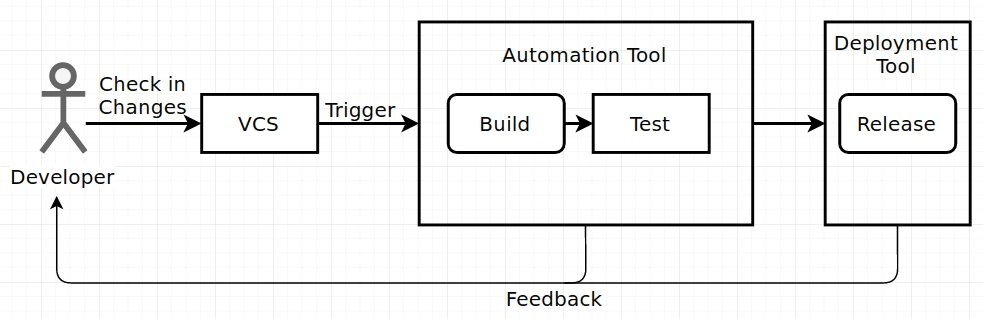
\includegraphics[scale=0.45]{images/pipeline-simple.jpg}
	\caption{The pipeline made simple}
	\label{fig:pipeline-simple}
\end{figure}

The developer will check in the code to the VCS witch in turn will trigger the automation tool. The automation tool will then build the project and test, before sending it out to release. If any of the stages fail the rest of the pipeline is not ran and feedback is sent to the developer so they can fix it.
\\\\
The testing part of the pipeline refers to unit tests and the other forms mentioned in the earlier chapters. Even on a full pass the feedback will be sent, this will help guard against false positives.
\\\\
When talking about the architecture such a system there are two side, firstly the software pipeline as seen above. How each of the steps flow into each over and what is needed to pass between each of the steps. The second is the hardware layout,  such as are the unit tests ran of the same server that it is built, or maybe the entire pipeline in confined to a single server.

\subsection{Software architecture}

Figure \ref{fig:pipeline-simple} showed a basic pipeline for a continuous delivery pipeline, however there is not enough details to build a system from this. Below figure \ref{fig:bsipipeline} shows the system developed from the project that sparked this paper:

\begin{figure}[H]
	\centering
	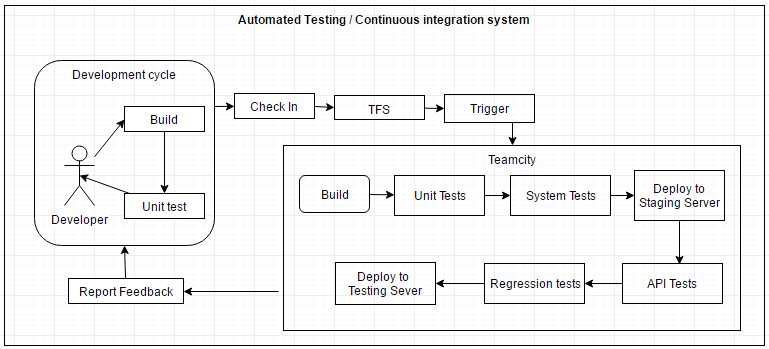
\includegraphics[scale=0.6]{images/bsipipleine.png}
	\caption{A full delivery pipeline}
	\label{fig:bsipipeline}
\end{figure}

The figure shows two things, firstly it reveals the local development cycle. The cycle being that the developer will check the basics before checking in the code to the VCS in this case a TFS server. Not noted on the diagram the developer will also have access to a local running copy of the program allowing them to run other forms of tests if needed. 
\\\\
The second part, it expands on the build and test block previously seen, firstly, the build, then the unit tests followed by system tests. System not mention before are tests a form of integration tests. This then leads on to a interesting part where the system is deployed on a staging instance, this allows the API and regression tests to be ran, as they require a the full system up and running. This is then deployed to testing  for manual tests, where it can then be pushed to production.
\\\\
The interesting part here is how four different deployments are needed, one for the developer, one for staging, one for testing and one for production. This is where Docker and other such tools fit into the picture.
\\\\
This kind of pipeline is a common one, some may use different types of tests as it will suite their needs better, but the theme is still the same. One such system by \cite{zend} adds an additional step after build to package the system up, ready to deploy, and as mentioned they have swapped out the test types for that which suit their product.
\\\\
Another interesting take on this by \cite{codeahoy}, has split their project into different components, this means rather than having one project to handle integration tests, both system to to be build and then integrated together. Therefore they used the architecture in figure \ref{fig:codeahoy}:

\begin{figure}[H]
	\centering
	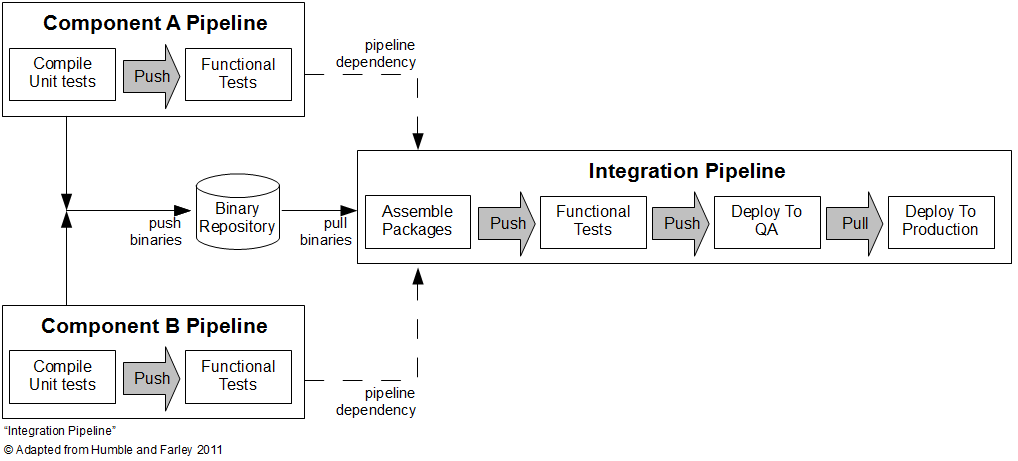
\includegraphics[scale=0.5]{images/codeahoy.png}
	\caption{A dual channel delivery pipeline by \cite{codeahoy}}
	\label{fig:codeahoy}
\end{figure}

This design has added an additional repository for binaries, then when a commit is placed in component A or B, it can progress through the entire pipeline by getting the latest version of the other components binaries from the repository. 
\\\\
\cite{thoughworks} takes this a step further by not only splitting the pipeline into separate components  but also places them in different repositories, making the first time they are integrated together being the integration tests as they all come from their own binary repositories.
\\\\
This kind of pattern goes along with the development environments based on breaking up a monolith architecture of a project into smaller more manageable units. This system makes it easy to add continuous deployment into micro service an other types of modular architecture.
\\\\
One thing not show so far but some teams find invaluable is to run a static analysis on the code base to pre-emptively spot erroneous areas in the project before they happen. This can then be sent back with the rest of the report to the developers and other interested parties.
\\\\
This basic pattern and flow of the pipeline does seems to be a common theme throughout all over implementations.  With the single monolith structure taking it from the start to end and the second combining multiple components into a single software package. 

\subsection{VCS workflow}

As seen the pipeline is generally triggered via a commit into the VCS this makes the workflow with the branch structure and VCS a central component into how the rest of the systems are put together.
\\\\
There are two main schools of thoughts when working with continuous deployment and VCS the first in more commonly seen in open source projects that are hosted on sites such as Github and Bitbucket, with the second when everyone has full access to the repository. 
\\\\
The fist uses a pull request system

\subsection{Hardware architecture}

\subsection{Architecture final words}
